\newcommand{\myname}{\textbf{A. del Val}}

\documentclass[12pt]{article}
\usepackage{sectsty}
%%%% Remove if not good %%%

\usepackage{geometry}
\usepackage{booktabs}
\usepackage{hyperref}
\geometry{a4paper, margin=1.1in, top=0.8in}

%%%%%%%
\usepackage{longtable}
\usepackage[most]{tcolorbox}
\definecolor{block-gray}{gray}{0.85}
\newtcolorbox{myquote}{colback=block-gray,boxrule=0pt,boxsep=0pt,breakable}
% \newtcolorbox{myquote}{colback=block-gray,grow to right by=-10mm,grow to left by=-10mm,
% boxrule=0pt,boxsep=0pt,breakable}
\makeatletter
\def\quoteparse{\@ifnextchar`{\quotex}{\singlequote}}
\def\quotex#1{\@ifnextchar`{\triplequote\@gobble}{\doublequote}}
\makeatother
\def\singlequote#1`{[StartQ]#1[EndQ]\quoteON}
\def\doublequote#1``{[StartQQ]#1[EndQQ]\quoteON}
\long\def\triplequote#1```{\begin{myquote}\parskip 1ex#1\end{myquote}\quoteON}
\def\quoteON{\catcode``=\active}
\def\quoteOFF{\catcode``=12}
\quoteON
\def`{\quoteOFF \quoteparse}
\quoteOFF

\pagenumbering{gobble}

\title{\large \textbf{SoFIA: So}bol-based sensitivity analysis, \textbf{F}orward and \textbf{I}nverse uncertainty propagation for \textbf{A}pplication to high temperature gases}
\date{}
\sectionfont{\fontsize{12}{15}\selectfont}
\begin{document}
\maketitle
% \thispagestyle{fancy}
\vspace{-2.5cm}
\begin{center}
\url{https://github.com/pysofia/SoFIA}\\
\vspace{0.5cm}
\textbf{Anabel del Val}\\
\vspace{0.5cm}
\date{\today} %25/06/2021
\end{center}

\section{Purpose and philosophy of this library}

This library was born out of my PhD studies. The code and tools initially available here are the ones I developed for my research. This library is not meant to be an exhaustive library such as \textit{scikit-learn} but a platform where I deposit my tools after cleaning them and making them more user-friendly. If you go online and type something like: UQ python, you'll find a myriad libraries so why developing my own? I also asked myself this question for a long time, and whenever possible, I used libraries that were already available. Libraries that are developed by a large group of individuals are generally better thought out, more efficient, more robust to changes, and they probably already have all you need. SoFIA is not a library for people wanting to do UQ in general. Other libraries are better. SoFIA is meant to fill-in the gap between the aerothermodynamics community and the UQ community.

Aerothermodynamicists in general have many other things to worry about in their research. We deal with complicated models and experimental facilities, and it is not often the case that we have the required mathematical background to do UQ. Therefore, looking for general purpose UQ libraries can be quite scary and burdensome. Our models are complex and so is our data. If you know me, you know that my PhD research was oriented towards developing UQ (in particular Bayesian) methodologies for their efficient use in aerothermodynamics models and experimental data. Based on that knowledge, I would assume you have come to SoFIA because whatever is in here will suit you as an aerothermodynamicist without the need to bend over backwards trying to understand those obscure mathematicians in search for a proper library.

I have often found libraries\footnote{In Python, although it also concerns other popular programming languages.} that do uncertainty propagation or Bayesian inference to be very naive. I'll explain myself. They generally use data formats that are only apt to be used with python functions. They assume the model you want to do UQ on is defined on python, which is generally not the case for our community. Working around these issues often require more work than just coding the whole thing yourself. Yes, such libraries have lots of modules and functionalities but it is not so worth to pay the price of having to adapt your model (that very complex code, made by many people's contributions over many years) to suit those libraries needs. That's the philosophy out of which SoFIA is conceived. It's true, there are other libraries, such as Sandia Labs' \textit{Dakota}\footnote{\url{https://dakota.sandia.gov}}, that are completely non-intrusive and can be a good fit for our needs. This is true, however, SoFIA also retains the possibility of defining your own model in python and using the library's methods without the need to encapsulate your code in an executable to work within \textit{Dakota}, speeding up the analyses in such cases. Further, SoFIA can also grow and adapt to your needs.

SoFIA contains the methods I needed to use during my PhD, nothing more. The methods are implemented in a way that it is very open to suit different models' needs. In general, SoFIA offers a workflow where you can generate samples of input variables that need to be used by the code of your choice. Then you can come back to SoFIA with the evaluations of the model and use other functionalities like computing Sobol indices or fitting a Gaussian Process model. SoFIA does not handle your model for you or ask you to format the model in a specific way. This is great for obtaining full flexibility while enjoying the library's methods.

Finally, the purpose of SoFIA is to also grow. If you happen to need to implement a new method, you can do so and merge it to the rest of SoFIA, so that the library keeps growing.

\section{Structure}

In within the SoFIA library, different modules are defined. This section is structured according to the different modules that can be found in SoFIA.\\

Create mind map or something and linkages to external functions and codes.

\section{Usage}

In this section, we describe the basic imports and object calls to use the different features of the SoFIA library.\\

\noindent\textbf{\small Probability distributions (\texttt{Probability\_distributions}).} This module can be found in \texttt{SoFIA/Probability\_distributions}. Several utilities are defined in \texttt{distributions}\texttt{.py}. There are two implementations: uniform distribution and Gaussian distribution. Both objects can be used with an arbitrary number of dimensions, although the resulting n-dimensional distributions do not account for correlation among variables. To instantiate a distribution object we prescribe the number of dimensions and the hyperparameters: lower and upper bounds for uniform distributions, and mean and standard deviation for Gaussian distributions. We can then compute PDF values, log-PDF values (useful for inverse problems), CDF values, inverse CDF values (to sample arbitrary distributions based on uniform or Gaussians), and sample from the distribution itself. A code snippet with a usage example is shown hereafter.\\

\quoteON
```
\texttt{import sofia.distributions as dist}\\

\texttt{hyp = [[a,b]] \# Hyperparameters for a 1D distribution}\\

\texttt{D = dist.Uniform(n\_dimensions,hyp) or dist.Gaussian(n\_dimensions,hyp) \# Instantiation of probability distribution object: either 1D uniform or Gaussian}\\

\texttt{x = np.linspace(-10.,10.,1000)}\\

\texttt{D.get\_cdf\_values(x) \# get CDF values of the distribution}\\

\texttt{D.get\_samples(n\_samples) \# Sample the distribution}

```
\quoteOFF

\noindent\textbf{\small Sensitivity Analysis (\texttt{SA}).} This module can be found in \texttt{SoFIA/SA}. In there, you can find the \texttt{Sobol.py} file with different utilities. We have the \texttt{sampling\_sequence} which generates the matrices with the inputs that need evaluations from our model, and \texttt{indices} which takes on the resulting evaluations and compute the first and total order Sobol' indices. You can print out the matrix with the inputs (each row contains all the inputs for one evaluation of the model) and then generate the evaluations the way you prefer. Then you come back and get your indices. The following code snippet shows an example of usage of this module. In \texttt{[...]} you can include the body of your code, namely, the function you want to perform sensitivity analysis on and any other relevant characteristics.\\
\quoteON
```
\texttt{import sofia.Sobol as sbl}\\

\texttt{[...] \# Definition of the function to be evaluated}\\

\texttt{SA = sbl.Sobol() \# Instantiation of sensitivity analysis object}\\

\texttt{samples = SA.sampling\_sequence(n\_samples,n\_variables,['dist vars'],None)}\\

\texttt{[...] \# Evaluation of function f on the samples computed}\\

\texttt{SA.indices(f,n\_samples,n\_variables)}

```
\quoteOFF

The concrete example with the Ishigami function can be found in \texttt{SA/example.py}.\\

\noindent\textbf{\small Inverse uncertainty propagation (\texttt{Iprop}).} This module is placed in \texttt{SoFIA/Iprop}. Utilities can be found in the script \texttt{sampler.py} with which a Markov chain based on the Metropolis Hastings algorithm can be built. For the instantiation of the sampler we have to specify an initial covariance function \texttt{covinit}, a loglikelihood function \texttt{fun\_in}, and the number of samples to burn for the adaptation of the covariance matrix \texttt{nburn}. The chain is initiated with the parameters specified in the utility \texttt{seed}, while the \texttt{Burn} routine adapts the covariance matrix with the presribed number of draws \texttt{nburn}. The function \texttt{DoStep} advances the Markov chain and generates the useful samples to be used in the analysis of the posterior distribution. The script \texttt{sampler.py} also includes two diagnostic techniques: the plotting of the trace through the \texttt{chain\_visual} function, and the computation of the autocorrelation function with \texttt{autocorr}. For the chain diagnostics object, we must specify the chain samples and a dictionary that links the position of the variables in the vector of variables used for the chain construction to a variable name for plotting purposes. A code snippet with the typical usage of this module is shown hereafter.\\

\quoteON
```
\texttt{import sofia.sampler as mcmc}\\

\texttt{[...] \# Model to be calibrated and corresponding definition of the loglikelihood function of the experiments}

\texttt{sampler = mcmc.metropolis(np.identity(n\_dim)*0.01, log\_lik, n\_samples) \# Instantiation of the MCMC sampler}\\

\texttt{[...] \# Definition of the initial values of the parameters to be calibrated}\\

\texttt{sampler.seed(initial\_values\_of\_parameters)}\\

\texttt{sampler.Burn()}\\

\texttt{for i in range(n\_samples):}\\
\texttt{sampler.DoStep(1)}\\

\texttt{sampler\_diag = mcmc.diagnostics(chain,dict\_var) \# Instantiation of the chain diagnostics object}\\

\texttt{sampler\_diag.chain\_visual(n\_plots,var)}\\

\texttt{sampler\_diag.autocorr(n\_lags,n\_plots,var)}

```
\quoteOFF

\noindent\textbf{\small Forward uncertainty propagation (\texttt{Fprop}).} Under development. For the moment, it includes a simple polynomial chaos construction. Sample-based methods can be built with the functionalities already included in the library. \\

\quoteON
```
\texttt{import sofia.pc as pce}\\
\texttt{import sofia.distributions as dist}\\

\texttt{\# Generate Gaussian samples to use}\\

\texttt{N = n\_samples}\\

\texttt{\# Definition of the distribution used in the PCE construction}\\

\texttt{hyp=[[0.,1.]]}\\
\texttt{G = dist.Gaussian(1,hyp)}\\
\texttt{S = G.get\_samples(N)}\\

\texttt{\# Definition of the targetted distribution}\\

\texttt{hypU=[[0.,1.]]}\\
\texttt{target = dist.Uniform(1,hypU)}\\

\texttt{h = target.fun\_icdf() \# Definition of the inverse CDF function of the target distribution}\\

\texttt{ki\_uniform = pce.approximate\_rv\_coeffs(n\_polynomials, h)}\\
\texttt{k = pce.generate\_rv(ki\_uniform, S) \# With k we should recover the target distribution}

```
\quoteOFF

\noindent\textbf{\small Applications (\texttt{Applications}).} Under development. It will include scripts with which to reproduce the results obtained in my PhD thesis. These scripts will put together different modules from SoFIA to perform all the computations. The only inputs to be provided will be the external model evaluations and inputs from which to construct Gaussian process surrogates and carry out the inverse and/or forward analyses. The data from the simulations I used in my thesis will also be available in another repository.\\

\section{Examples}

Particular examples of the usage of the different modules depicted in the previous section can be found in \texttt{SoFIA/examples}. Here we describe some of them and show the results for verification purposes.\\

\noindent \textbf{\small Probability distributions (\texttt{Probability\_distributions}).} In the example \texttt{Probability} \texttt{\_distributions}\texttt{/examples/example.py} we compute 1D and 2D uncorrelated uniform and Gaussian distributions. We first sample a uniform distribution with support $\mathcal{U}[-8,8]$ for which we generate 1000 samples and compute the CDF and PDF.

\begin{figure}[!htb]
    \centerline{
    \begin{tabular}{c c}
    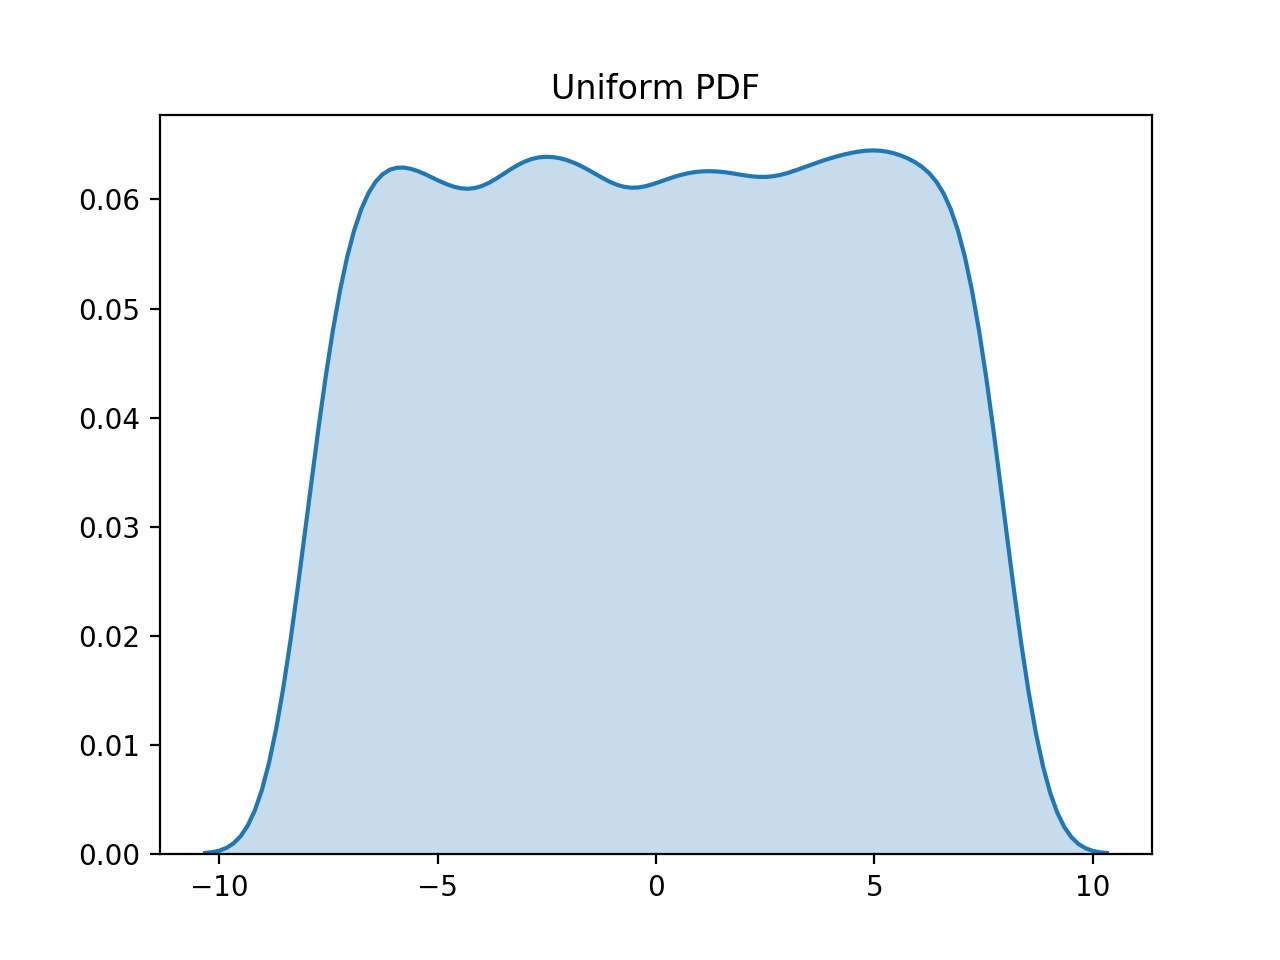
\includegraphics[width=0.5\textwidth]{./figures/uniform_pdf.png} &
    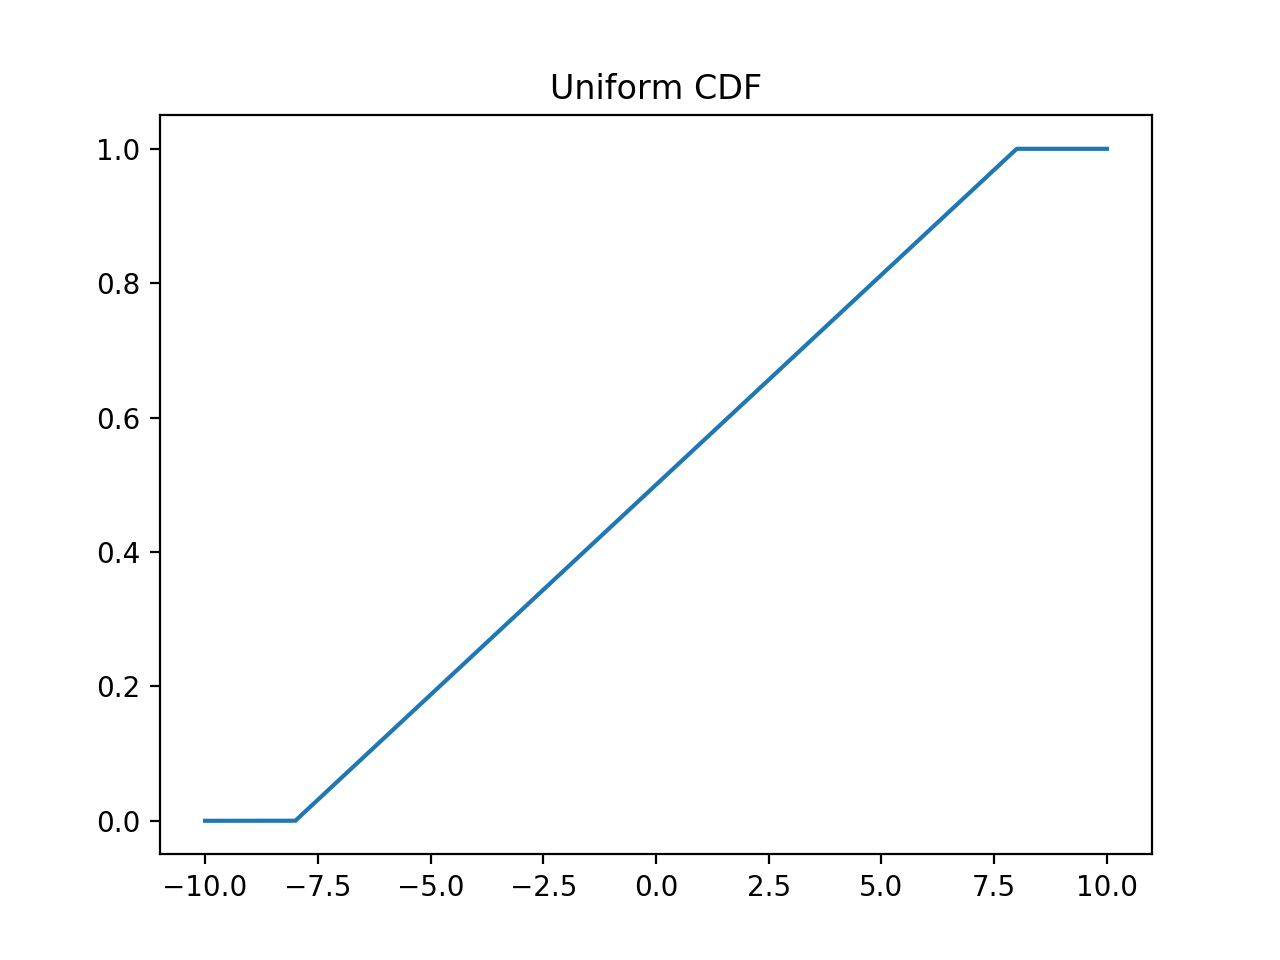
\includegraphics[width=0.5\textwidth]{./figures/uniform_cdf.png} 
    \end{tabular}}
    \caption{1D uniform PDF and CDF.}
    \label{fig:1d_uniform}
\end{figure}

We do the same for a 1D Gaussian distribution $\mathcal{N}(\mu=-1, \sigma=4)$

\begin{figure}[!htb]
    \centerline{
    \begin{tabular}{c c}
    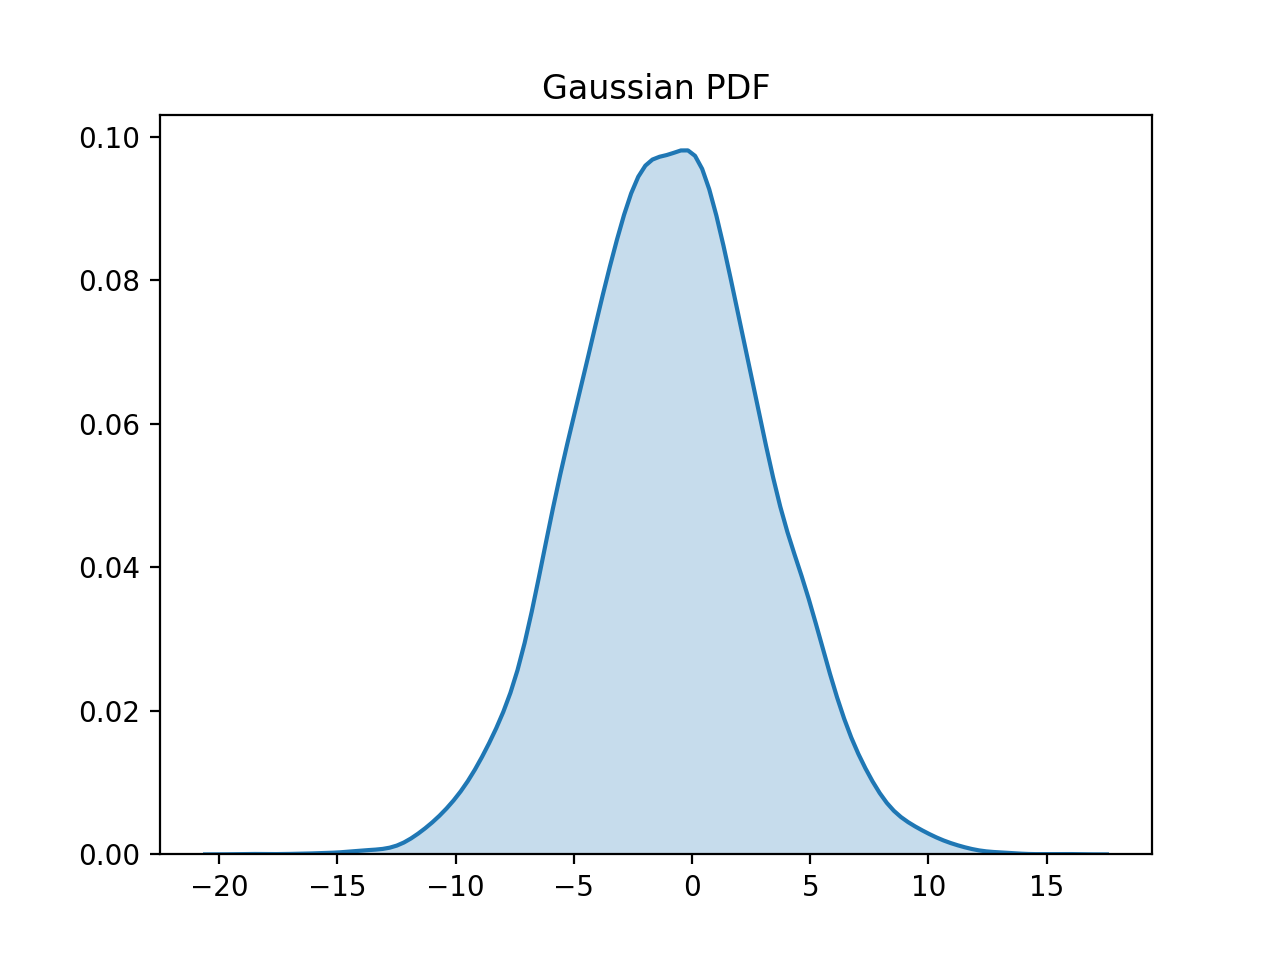
\includegraphics[width=0.5\textwidth]{./figures/gaussian_pdf.png} &
    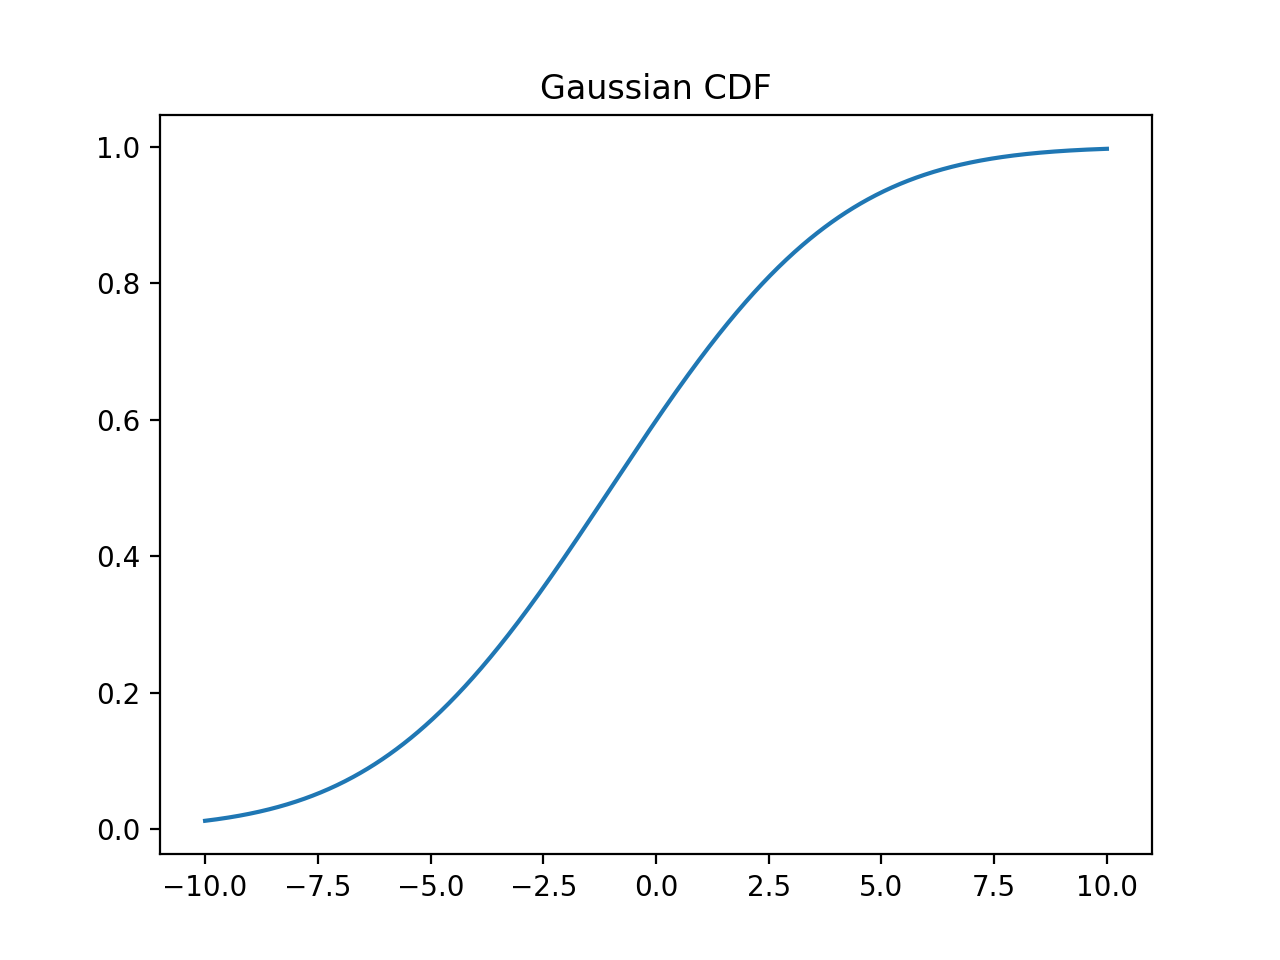
\includegraphics[width=0.5\textwidth]{./figures/gaussian_cdf.png} 
    \end{tabular}}
    \caption{1D Gaussian PDF and CDF.}
    \label{fig:1d_gaussian}
\end{figure}

We can also compute marginal CDFs and PDFs for 2D distribution of uncorrelated variables. In this case, the uniform distribution has for hyperparameters $\mathcal{U}[-1,4] \times \mathcal{U}[0,2]$, while the 2D Gaussian is defined $\mathcal{N}(-1,4) \times \mathcal{N}(0,2)$.\\

\begin{figure}[!htb]
    \centerline{
    \begin{tabular}{c c}
    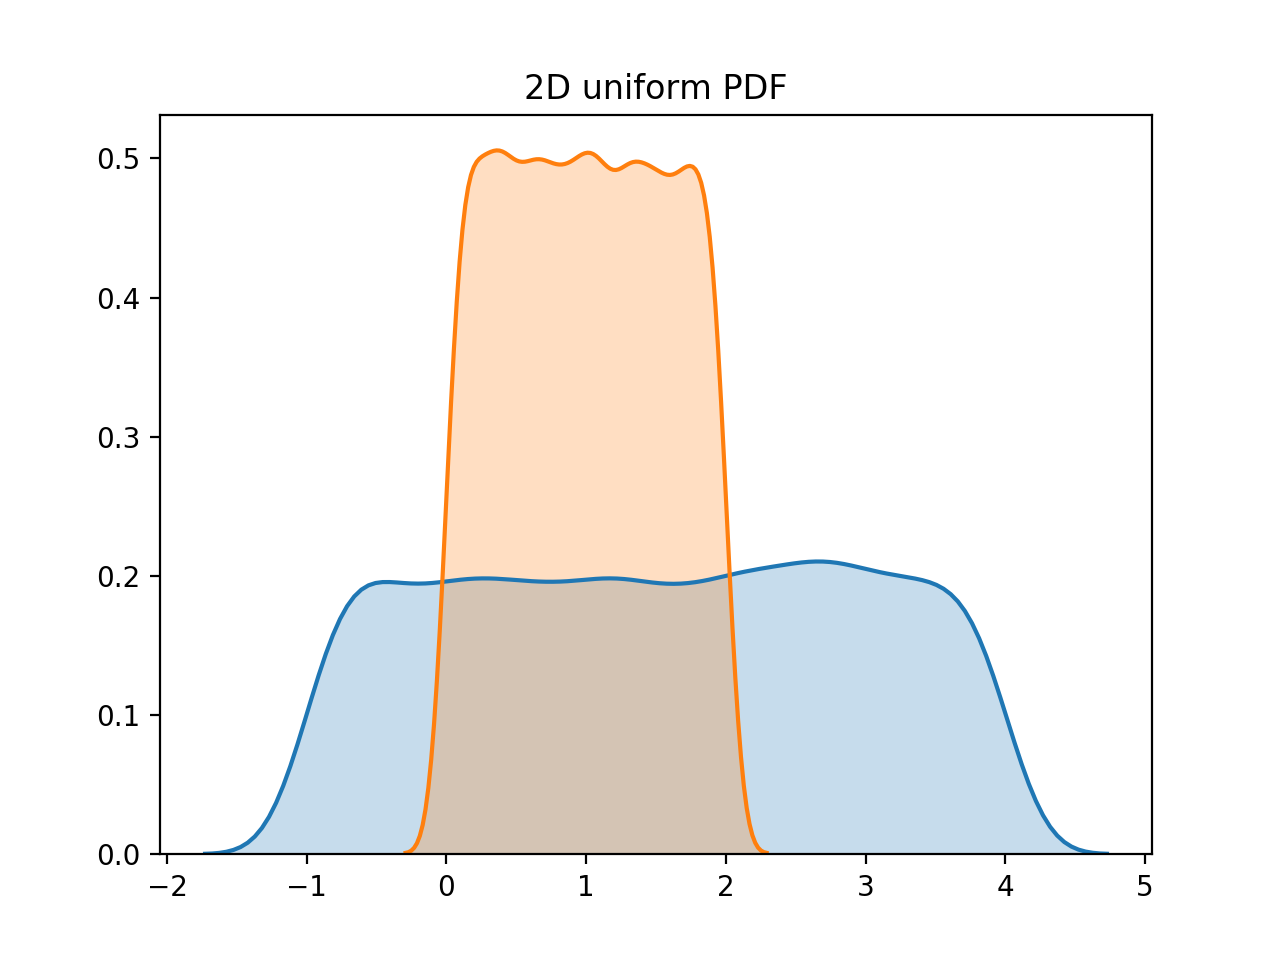
\includegraphics[width=0.5\textwidth]{./figures/marginal_uniform_pdf.png} &
    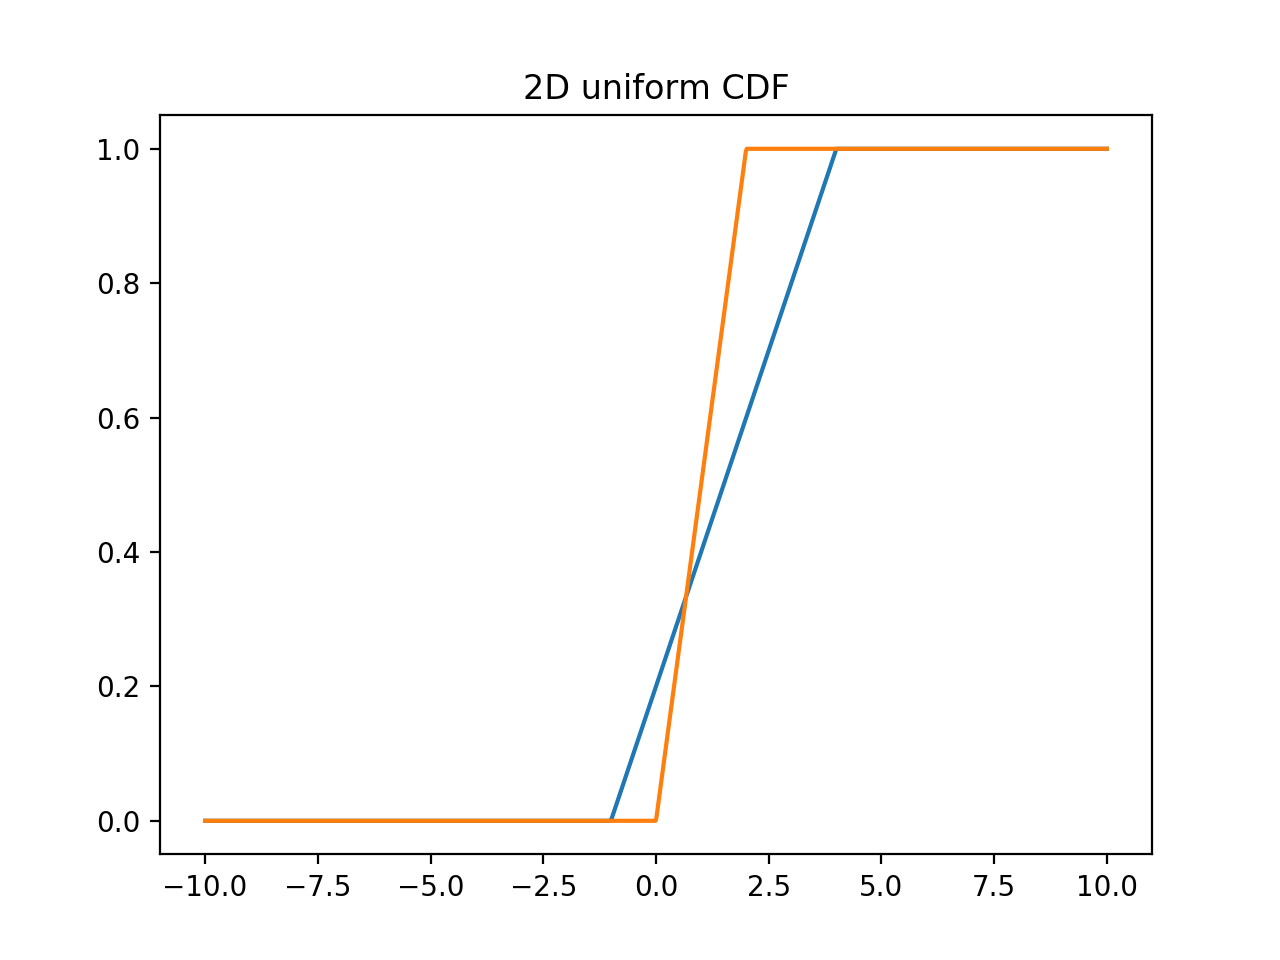
\includegraphics[width=0.5\textwidth]{./figures/marginal_uniform_cdf.png} \cr
    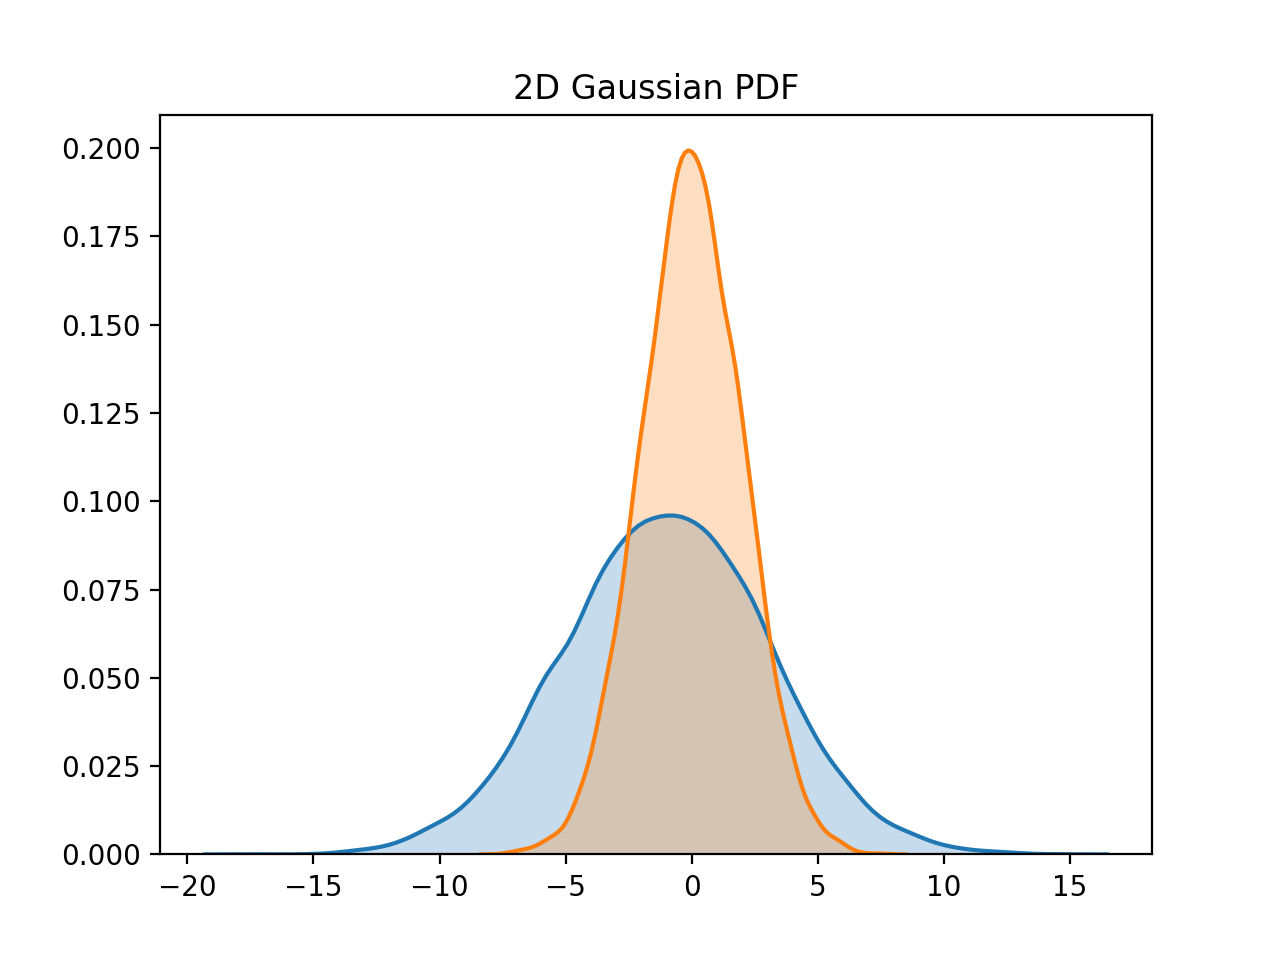
\includegraphics[width=0.5\textwidth]{./figures/marginal_gaussian_pdf.png} &
    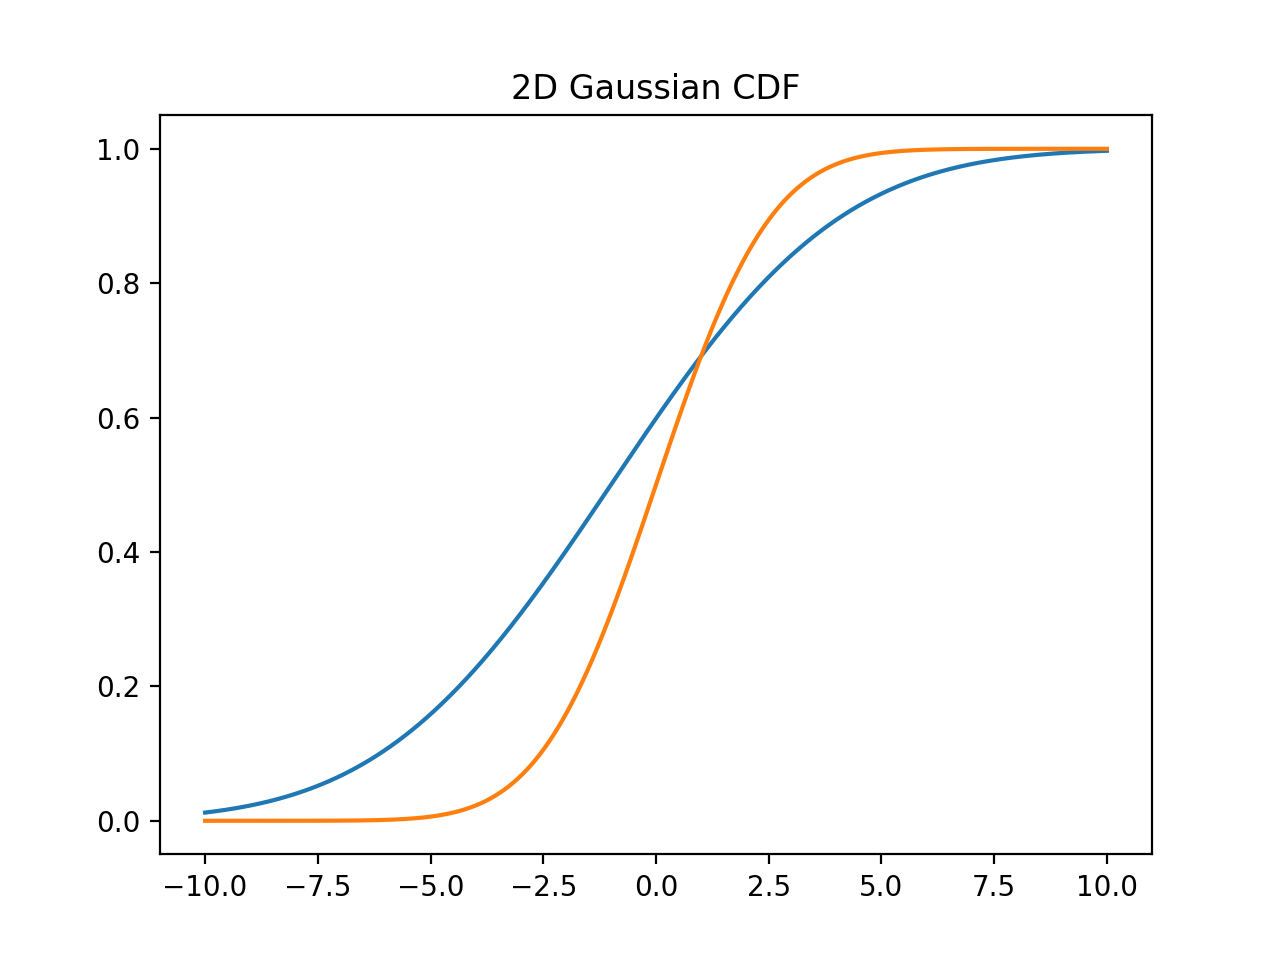
\includegraphics[width=0.5\textwidth]{./figures/marginal_gaussian_cdf.png}
    \end{tabular}}
    \caption{2D uniform and Gaussian marginal PDFs and CDFs.}
    \label{fig:1d_gaussian}
\end{figure}

\noindent \textbf{\small Sensitivity Analysis (\texttt{SA}).} In the example \texttt{SA/examples/example.py}, we work with the Ishigami function\\

\begin{equation}\label{eq:ishigami}
    f(x,y) = \sin(x) + a \cdot \sin(y)^{2} + b \cdot z^{4}\sin(x),
\end{equation}
for which we compute sensitivity indices for $x, y, z$ with respect to the model output $f$. The model parameters $a$ and $b$ are set to the values 7 and 0.1, respectively. We assume uniform distributions $\mathcal{U}[-\pi,\pi]$ for $x, y, z$ and base our estimations on 10,000 samples.

\begin{table}[!hbt]
    \centering
    \caption{Sobol' sensitivity indices for the inputs $x, y, z$ of the Ishigami function~\eqref{eq:ishigami}.} 
    \label{tab:models}
      \begin{tabular}{c  c  c}
        \toprule
        Variables  & $S_{i}$  & $S_{\mathrm{T}_{i}}$ \\ \midrule
        $x$ & 0.312 & 0.576\\
        $y$ & 0.446 & 0.443\\
        $z$ & 0.009 & 0.246\\
    
      \end{tabular}
\end{table}

\noindent \textbf{\small Inverse uncertainty propagation (\texttt{Iprop}).} There are several examples for this module. \\

\noindent\textbf{\small Example 1.} The first example \texttt{Iprop/examples/example\_ishigami.py} consists of inferring parameters $a$ and $b$ from noisy observations $f$ of the Ishigami function~\eqref{eq:ishigami}. In this case, the parameters are set to the values $a=8$ and $b=1$ while the noise of the observations is set to $\sigma=0.2$. The results are based on data in 3 different points $(x,y,z)$: $(0,1,2), (0,2,5)$, and $(1,8,5)$. The following figure~\ref{fig:ishigami_inverse} shows the trace for parameter $b$ and the marginal posteriors obtained for a 100,000 steps chain with an initial burn-in stage of 100,000 samples. The overall acceptance rate is 0.34008.

\begin{figure}[!htb]
    \centerline{
    \begin{tabular}{c c}
    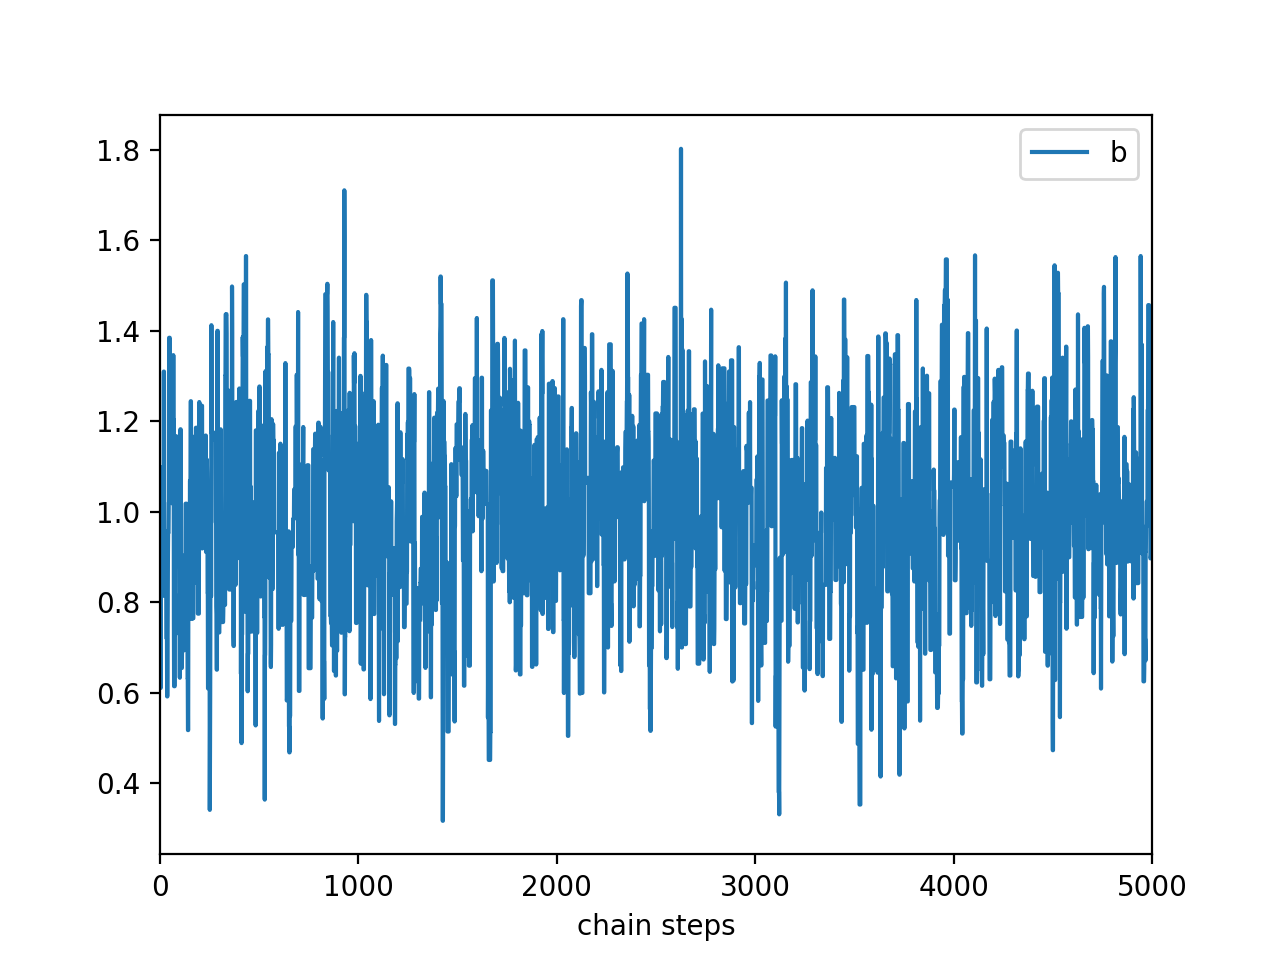
\includegraphics[width=0.5\textwidth]{./figures/ishigami_chain_trace.png} &
    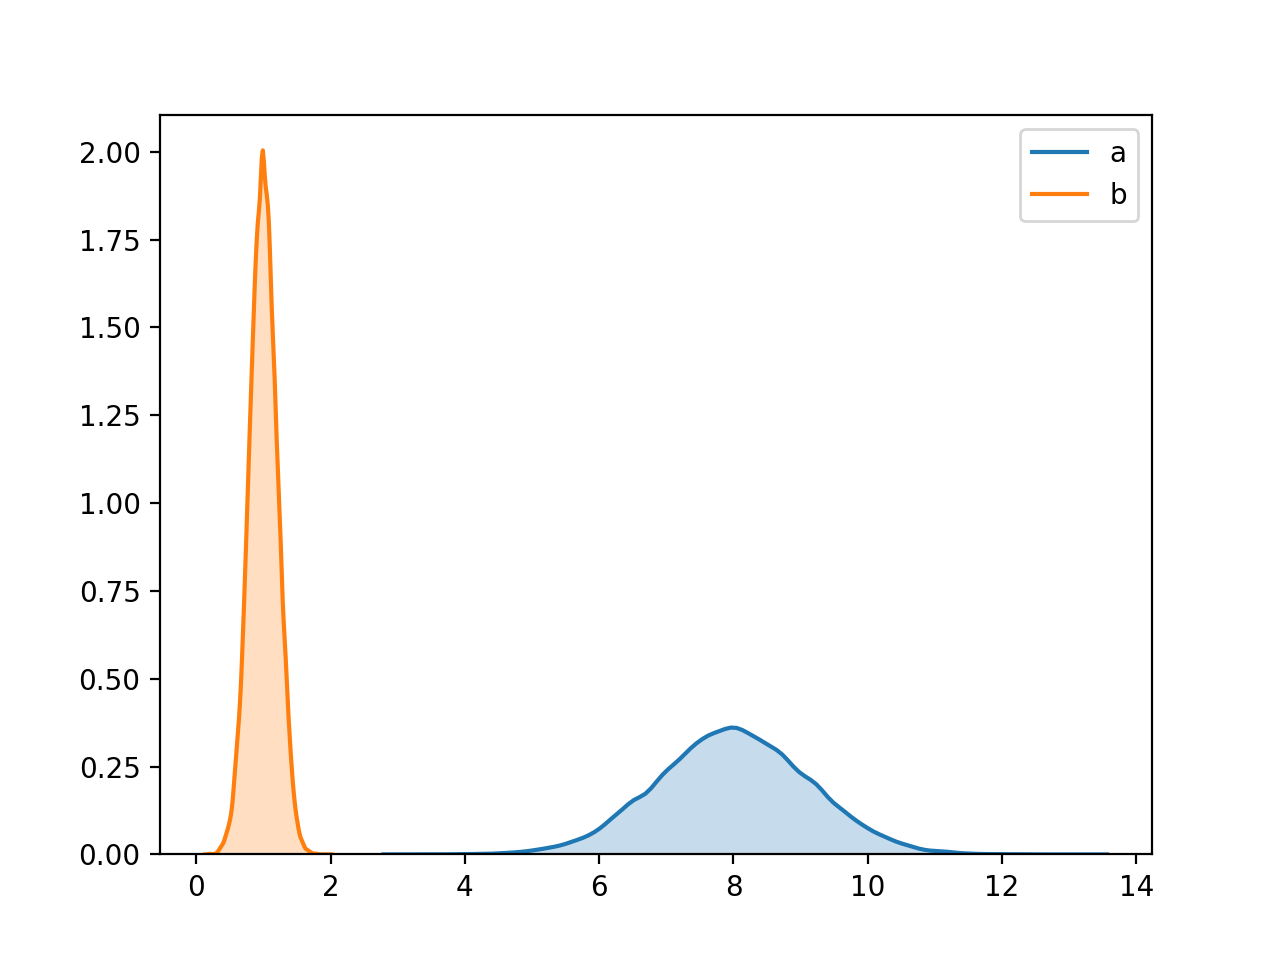
\includegraphics[width=0.5\textwidth]{./figures/ishigami_marginal_post.png}
    \end{tabular}}
    \caption{Left: chain trace for parameter $b$ for 5,000 steps. Right: marginal posterior distributions of parameters $a$ and $b$.}
    \label{fig:ishigami_inverse}
\end{figure}

We also show the autocorrelation function in the following figure

\begin{figure}[!htb]
    \centerline{
    \begin{tabular}{c c}
    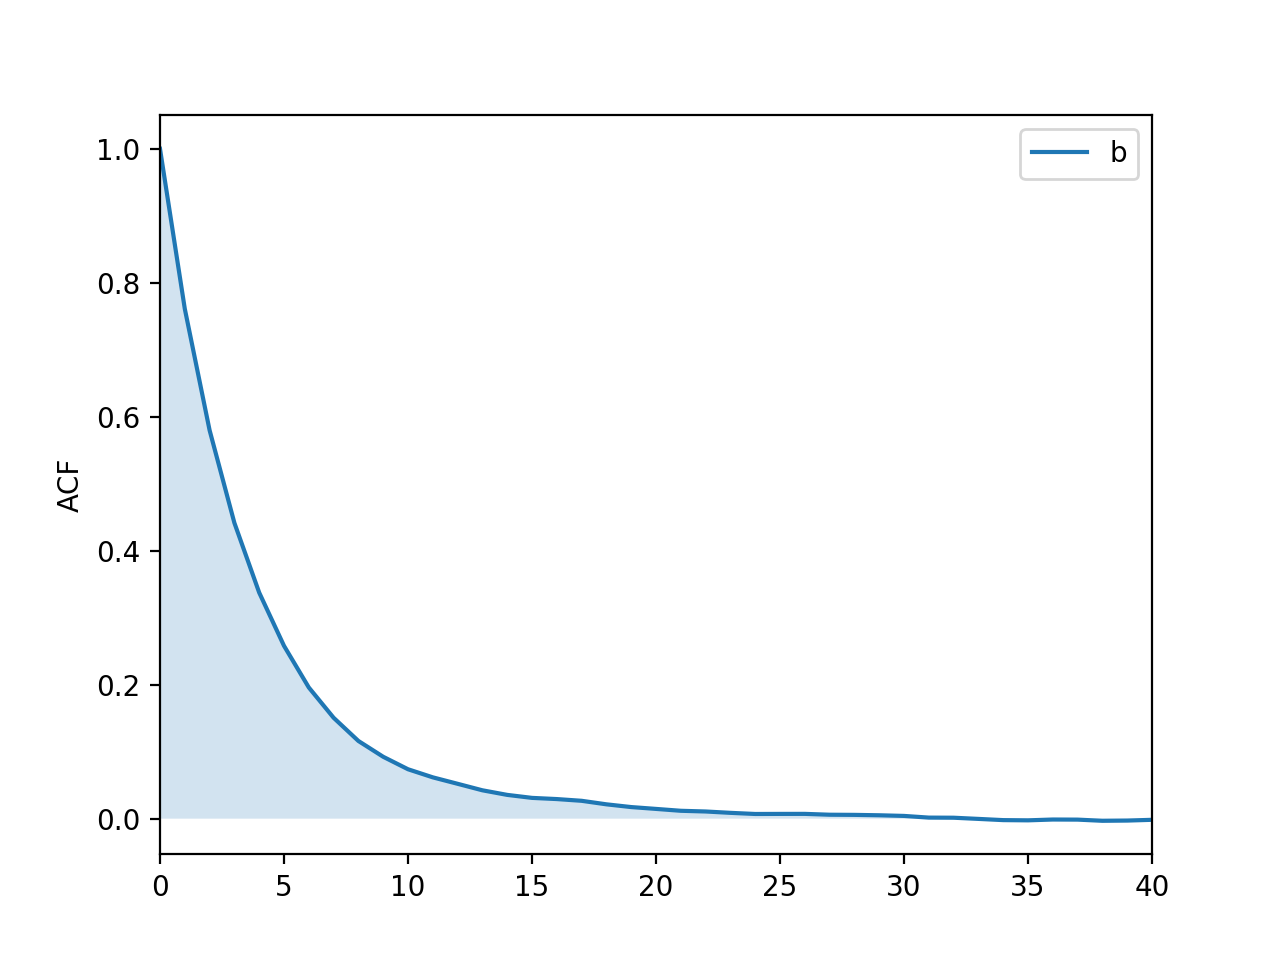
\includegraphics[width=0.5\textwidth]{./figures/ishigami_acf.png}
    \end{tabular}}
    \caption{Autocorrelation function of the chain for parameter $b$.}
    \label{fig:ishigami_acf}
\end{figure}

\noindent\textbf{\small Example 2.} Another example consists on the sampling of two Gaussian distributions by means of MCMC. We sample the Gaussians $\mathcal{N}(0,1)$ and $\mathcal{N}(5,1)$ whose true analytical PDFs are compared to the MCMC result through which the mean parameters $\mu_{1}$ and $\mu_{2}$ of the distributions are estimated. Figs~\ref{fig:mcmc_gaussian_pdf}-\ref{fig:mcmc_gaussian_chain_acf} show the results.

\begin{figure}[!htb]
    \centerline{
    \begin{tabular}{c c}
    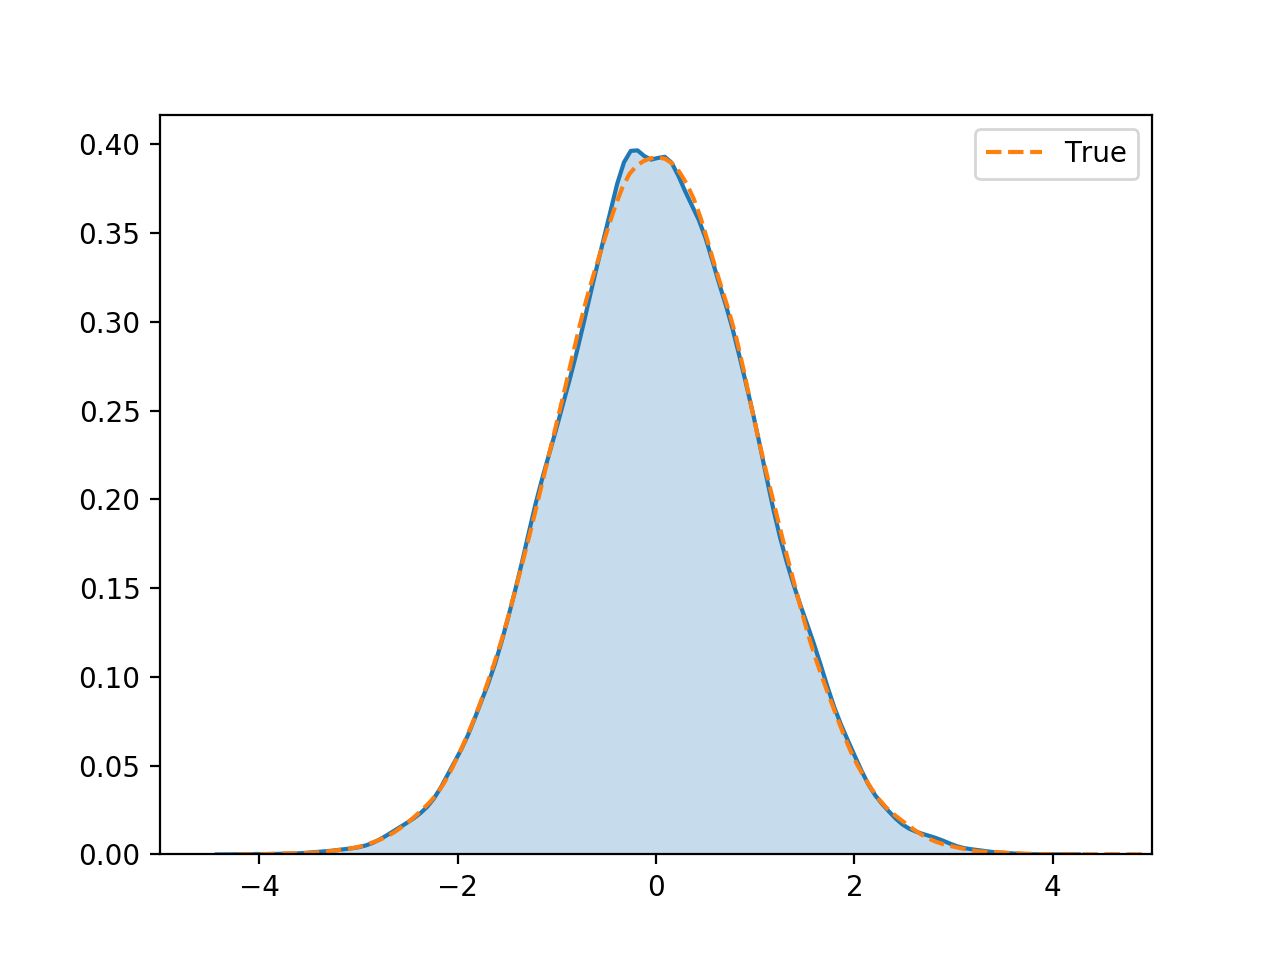
\includegraphics[width=0.5\textwidth]{./figures/mcmc_N01.png} &
    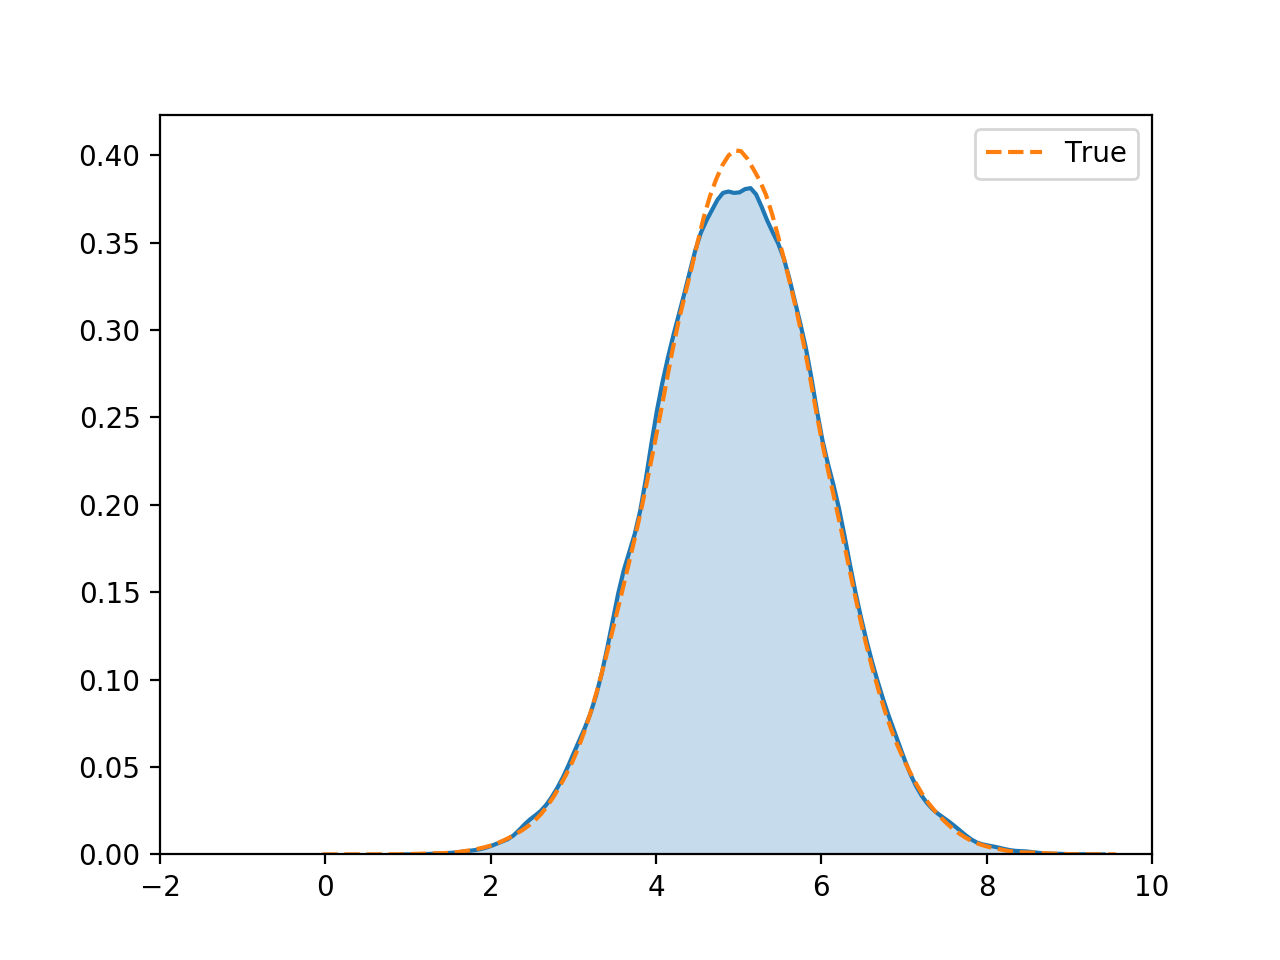
\includegraphics[width=0.5\textwidth]{./figures/mcmc_N51.png}
    \end{tabular}}
    \caption{Left: true PDF versus the PDF recovered from the Markov chain samples for the first Gaussian distribution $\mathcal{N}(0,1)$ Right: true PDF versus the PDF recovered from the Markov chain samples for the first Gaussian distribution $\mathcal{N}(5,1)$.}
    \label{fig:mcmc_gaussian_pdf}
\end{figure}

\begin{figure}[!htb]
    \centerline{
    \begin{tabular}{c c}
    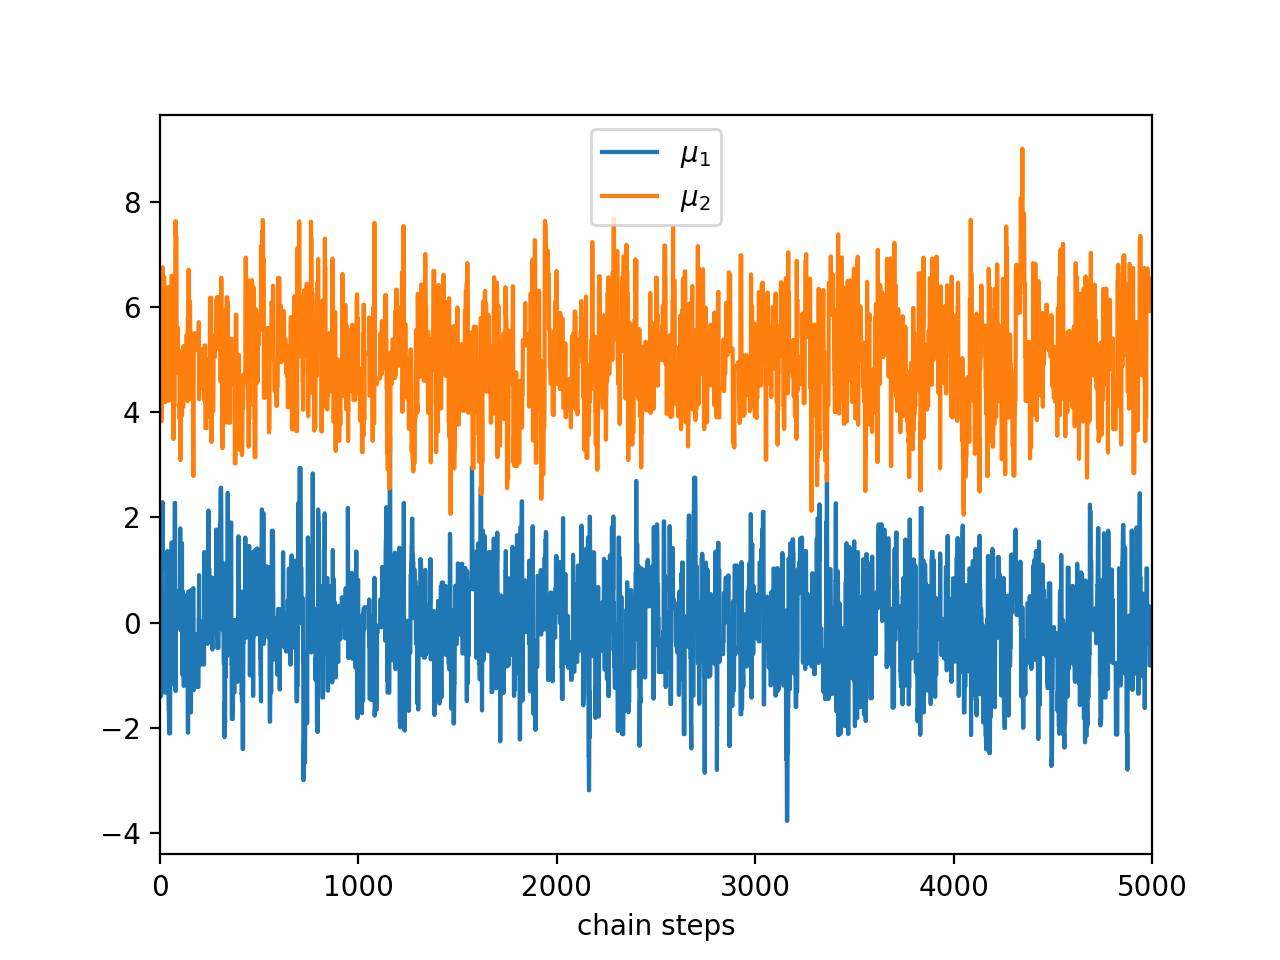
\includegraphics[width=0.5\textwidth]{./figures/mcmc_gaussian_chains.png} &
    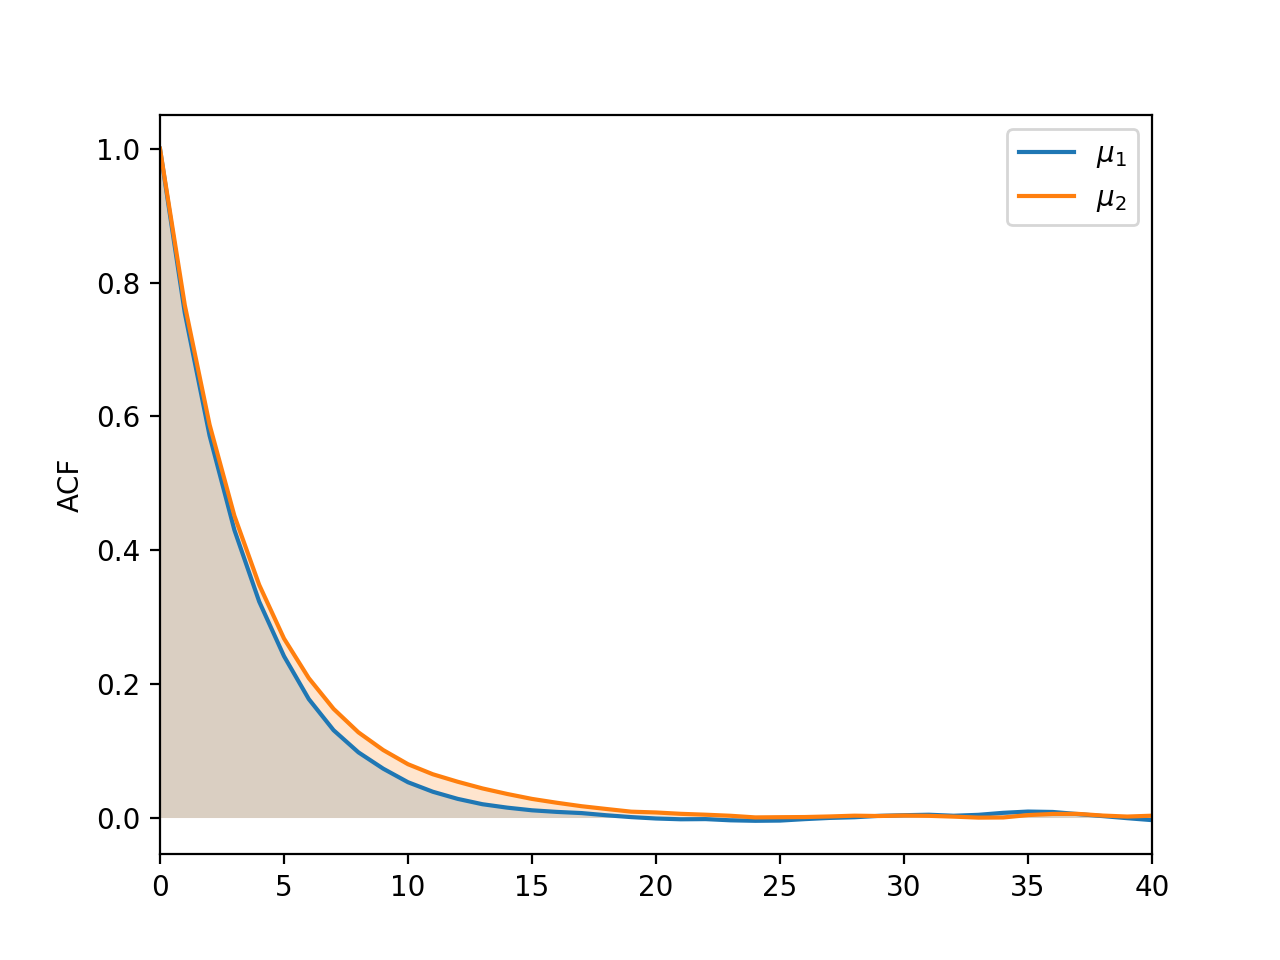
\includegraphics[width=0.5\textwidth]{./figures/mcmc_gaussian_acfs.png}
    \end{tabular}}
    \caption{Left: chain traces for parameters $\mu_{1}$ and $\mu_{2}$ of the Gaussian distributions we are sampling with a MCMC method for 5,000 steps. Right: autocorrelation functions.}
    \label{fig:mcmc_gaussian_chain_acf}
\end{figure}

\noindent\textbf{\small Example 3.} The last example included in the library consists of the reconstruction of a polynomial of arbitrary degree $k$, $f(x) = \sum_{k=0}^{q} a_{q}x^{q}$ from 30 noisy observations randomly sampled in the canonical range $x \in [0,1]$ with $\sigma=0.1$. We first fit the linear polynomial 

\begin{equation}
    f(x) = 10 -2 \cdot x
\end{equation}
by fixing $a_{0} = 10$, $a_{1} = -2$ and $a_{i} = 0, \ \ \forall i \in {2,...,4}$. The results of the posterior predictive check as well as the marginal posteriors of the parameters are shown in Fig.~\ref{fig:poly_lin}.

\begin{figure}[!htb]
    \centerline{
    \begin{tabular}{c c}
    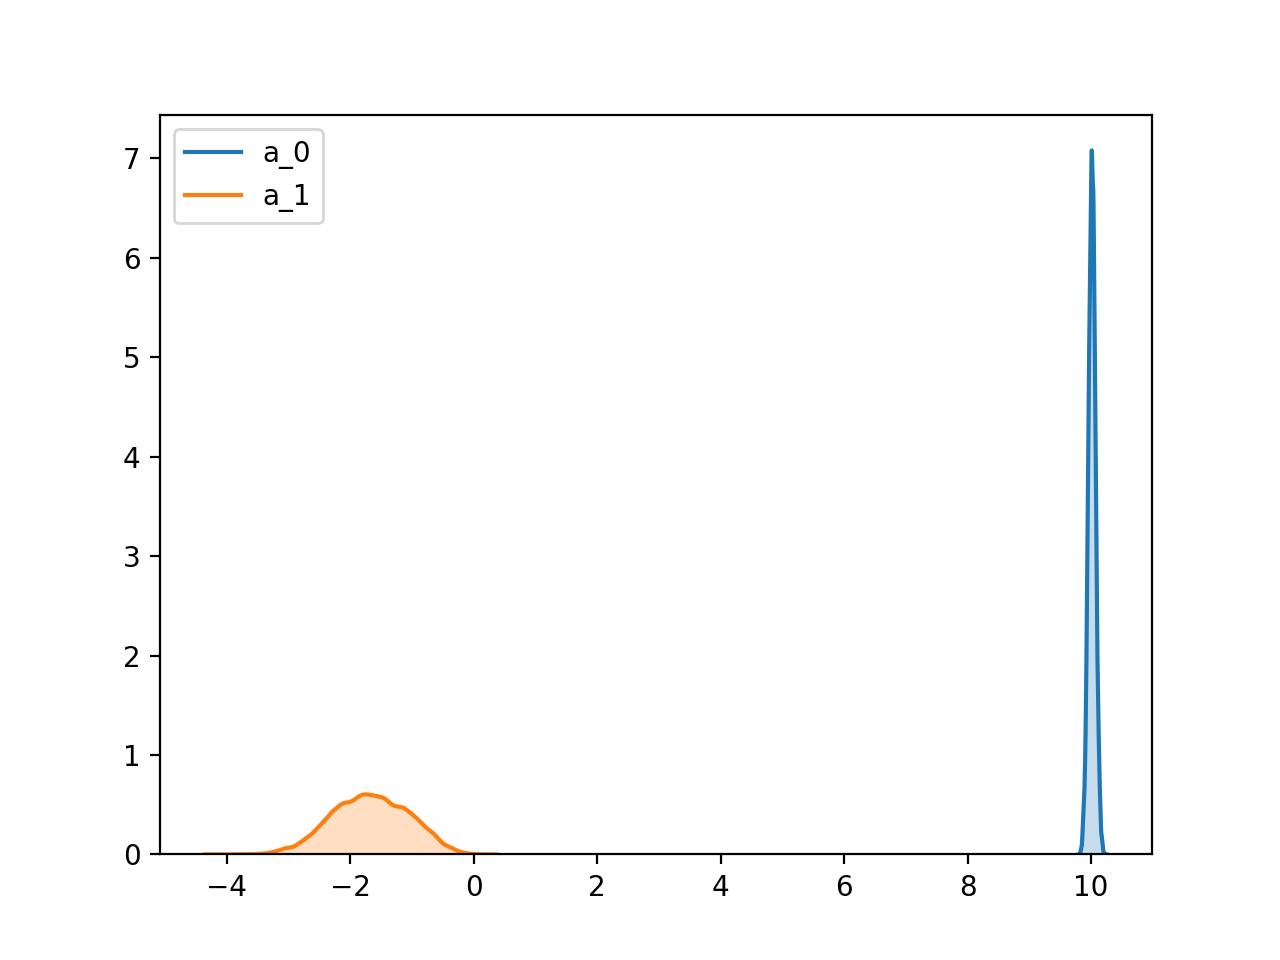
\includegraphics[width=0.5\textwidth]{./figures/linear_coeffs.png} &
    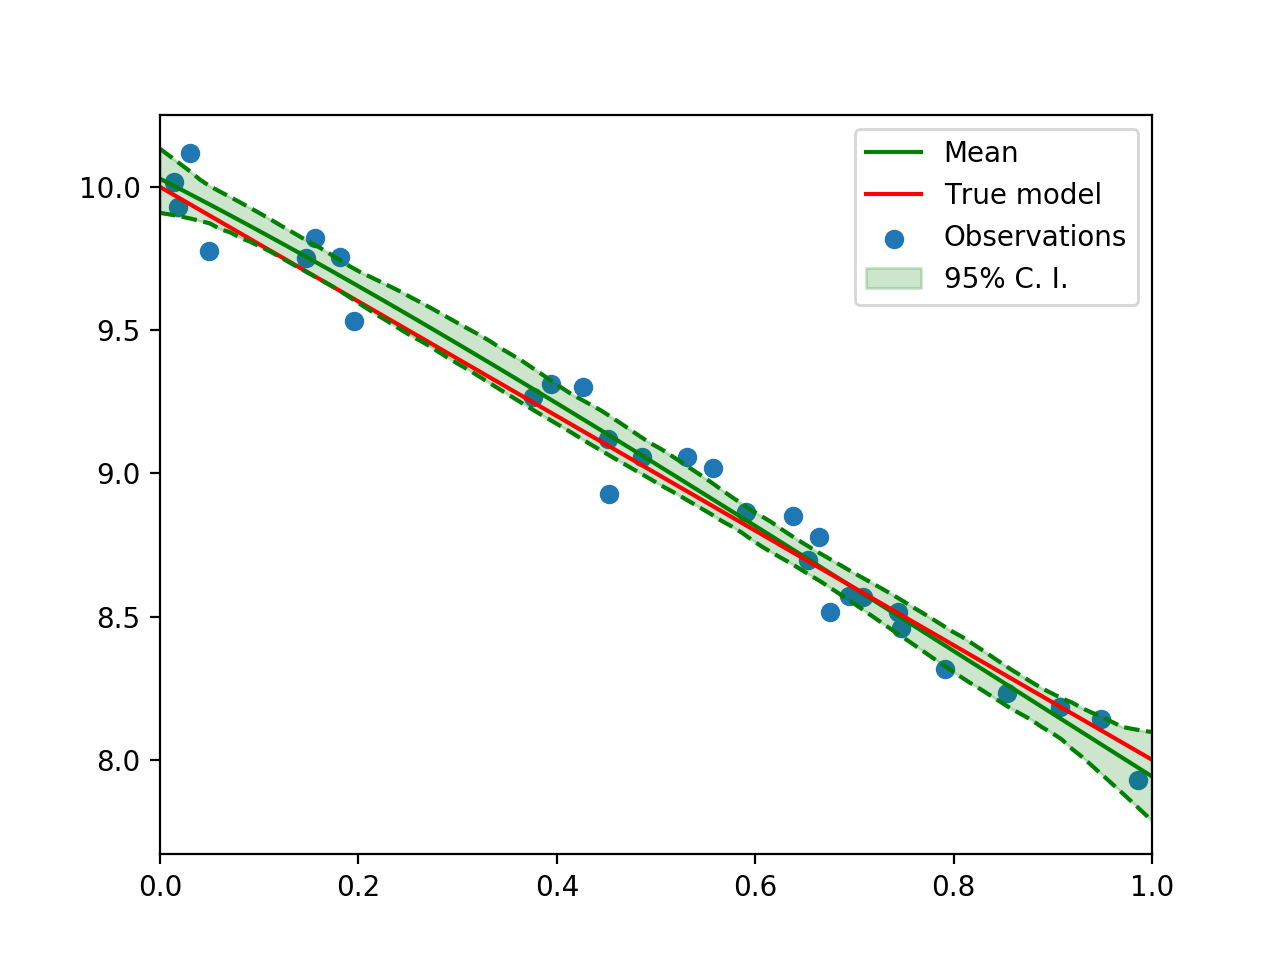
\includegraphics[width=0.5\textwidth]{./figures/linear_polynomial.png}
    \end{tabular}}
    \caption{Left: marginal posterior distributions for parameters $a_{0}$ (bias) and $a_{1}$ (slope) for the linear polynomial model. Right: posterior predictive check.}
    \label{fig:poly_lin}
\end{figure}

We then fit a more challenging model, $f(x) = 10 - 2 \cdot x + 7.5 \cdot x^{2} - 3.3 \cdot x^{3} - 3.2 \cdot x^{4}$ with the results shown in Fig.~\ref{fig:poly}. Parameter $a_{0}$ has been omitted from the marginal posteriors given the more peaky behavior compared to the rest of the parameters, giving poor viasualization of the results when plotted all together. $a_{0}$ marginal posterior closely resembles that of Fig.~\ref{fig:poly_lin}.\\

\begin{figure}[!htb]
    \centerline{
    \begin{tabular}{c c}
    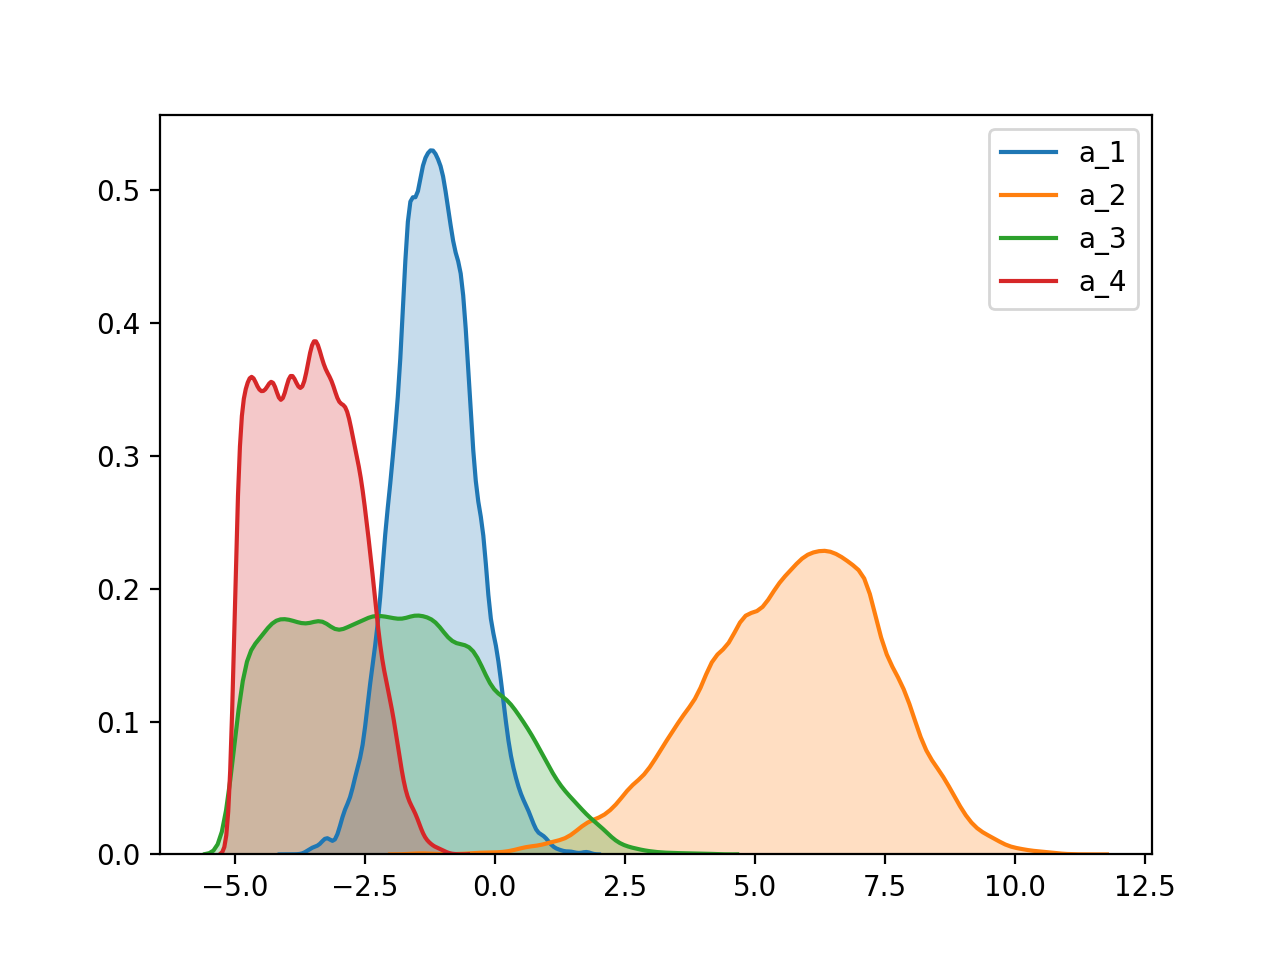
\includegraphics[width=0.5\textwidth]{./figures/poly_posteriors_m0.png} &
    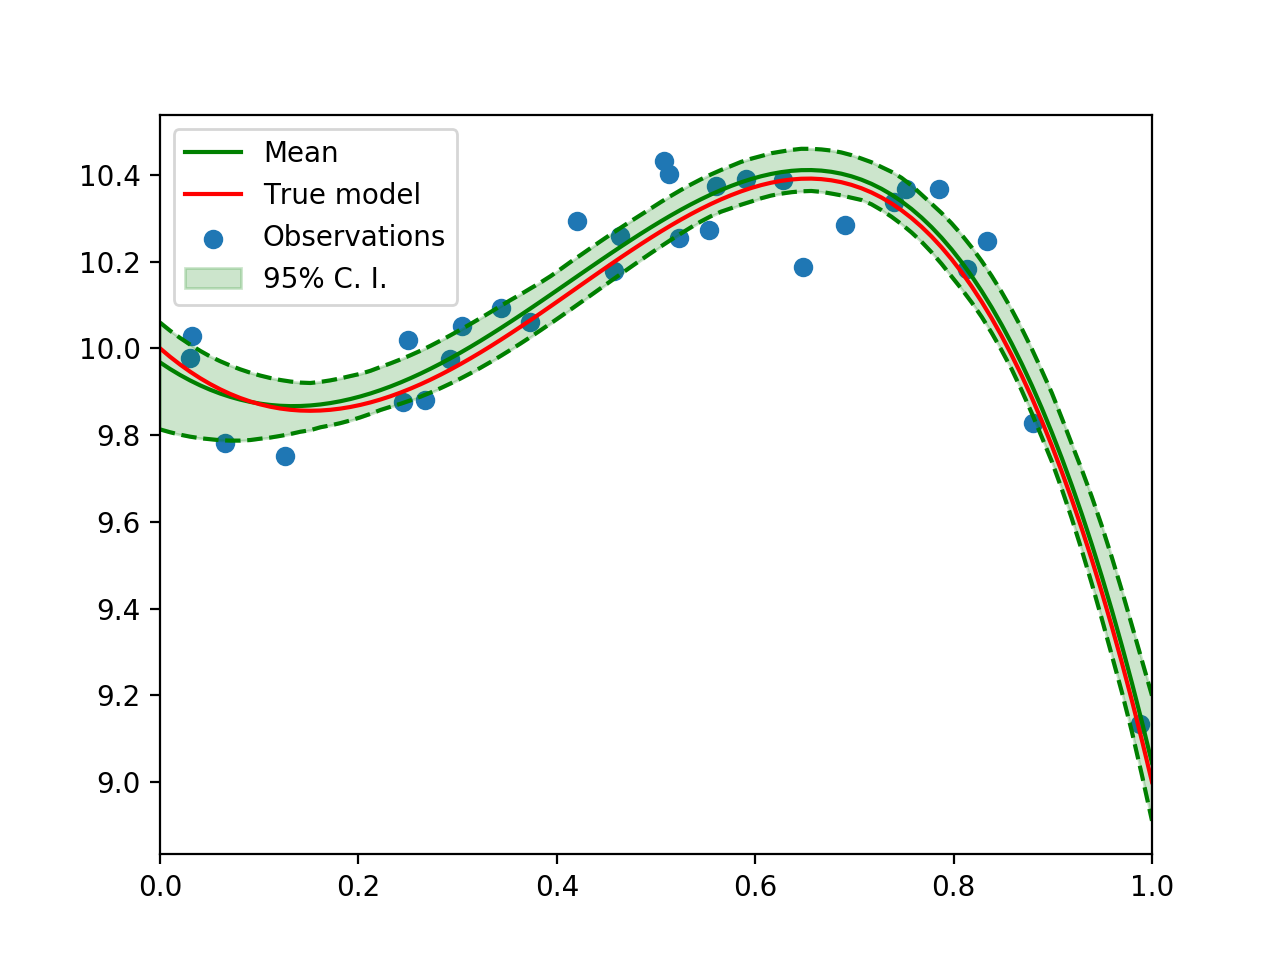
\includegraphics[width=0.5\textwidth]{./figures/poly_predict_check.png}
    \end{tabular}}
    \caption{Left: marginal posterior distributions for parameters $a_{1,...,4}$ for the polynomial model. Right: posterior predictive check.}
    \label{fig:poly}
\end{figure}

\noindent \textbf{\small Forward uncertainty propagation (\texttt{Fprop}).} In this module, we include a simple polynomial chaos construction. The example included is the polynomial chaos expansion of a uniform distribution based on canonical Gaussian distributions $\mathcal{N}(0,1)$. \\

\noindent \textbf{\small Applications (\texttt{Applications}).} Adiabatic reactor with Mutation++\\

\noindent \textbf{\small Adiabatic reactor.} In this example, we use the python implementation of the physico-chemical library Mutation++\footnote{\url{https://github.com/mutationpp/Mutationpp}} to compute the time evolution of the temperature for an air5 $\{\mathrm{N, NO, O, O_{2}, N_{2}}\}$ adiabatic reactor. The results in terms of the Sobol indices evolution with time is shown in Fig.~\ref{fig:ad_react_SA}. In the legend, the chemical mechanism considered for such mixture is shown.

\begin{figure}[!htb]
    \centering{
    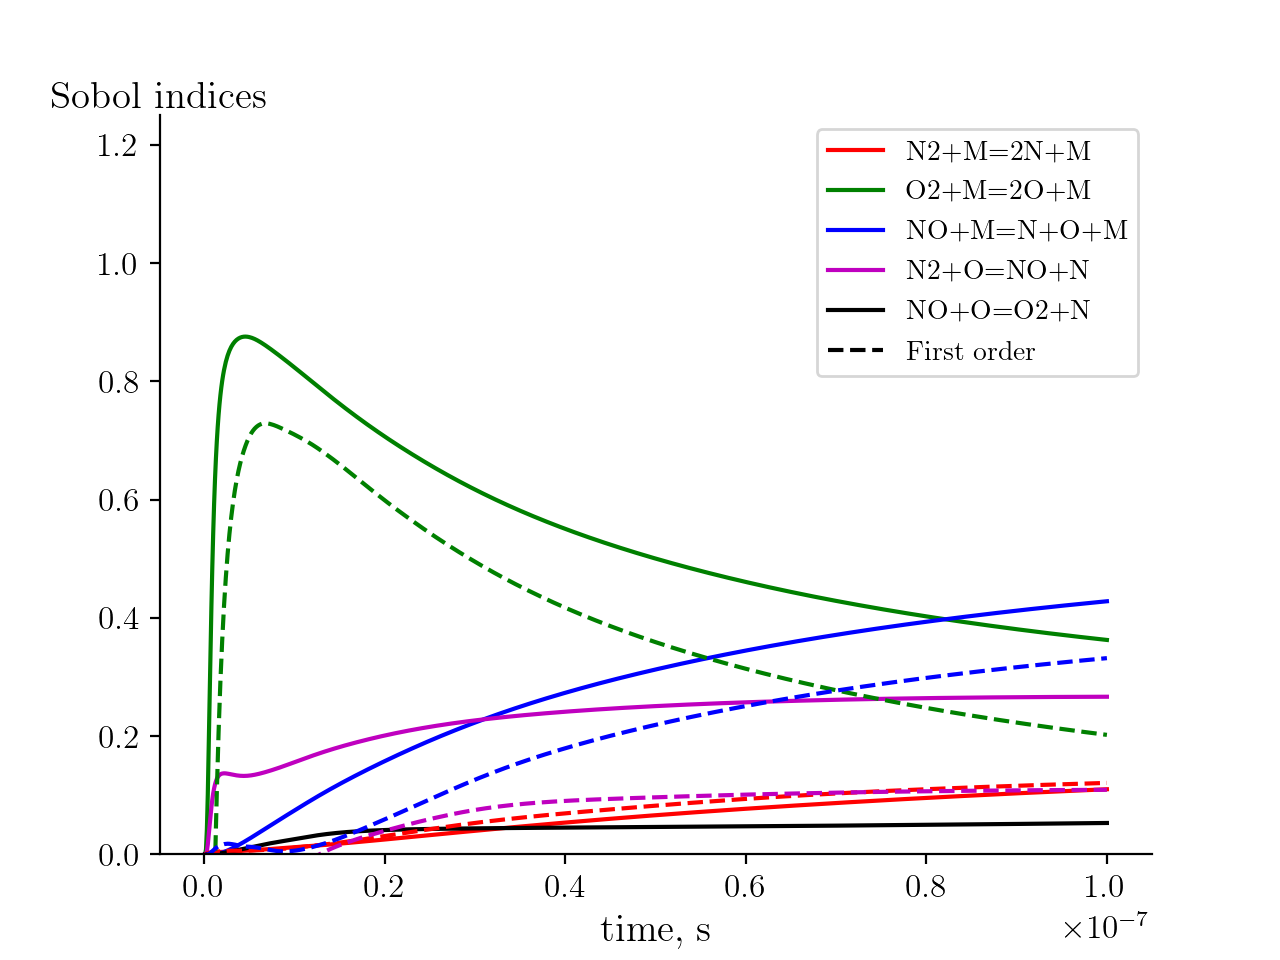
\includegraphics[width=0.7\textwidth]{./figures/Sobol_10000.png}
    \caption{Time evolution of the first order and total order Sobol indices for the variance-based sensitivity of the temperature evolution of an air5 adiabatic reactor at 100 hPa with respect to the pre-exponential factors of the reaction rates of the chemical mechanism.}}
    \label{fig:ad_react_SA}
\end{figure}

For such example, the reaction rates were sampled from log-uniform distributions with the hyperparameters shown in Table~\ref{tab:react_dist}. They have been chosen to encompass their current value according to the chemical model of Park, and also with a variability that does not produce instabilities in the solver in Mutation++. The Sobol indices are based on a Monte Carlo estimate with 10,000 samples. This example is just to demonstrate how SoFIA can be coupled to other libraries to produce various results. The implementation has been sped-up by using parallelization via the module \texttt{mpi4py}.

\begin{table}[!hbt]
    \centering
    \caption{Probability distributions for the pre-exponential factors of the reaction rates of an air5 chemical mechanism.} 
    \label{tab:react_dist}
      \begin{tabular}{l  l}
        \toprule
        Variables  & distribution \\ \midrule
        $\log A_{\mathrm{N_{2}+M \rightleftharpoons 2N+M}}$ & $\mathcal{U}[20,22]$ \\
        $\log A_{\mathrm{O_{2}+M \rightleftharpoons 2O+M}}$ & $\mathcal{U}[20,22]$ \\
        $\log A_{\mathrm{NO+M \rightleftharpoons N+O+M}}$ & $\mathcal{U}[10,15]$ \\
        $\log A_{\mathrm{N_{2}+O \rightleftharpoons NO+N}}$ & $\mathcal{U}[10,15]$ \\
        $\log A_{\mathrm{NO+O \rightleftharpoons O_{2}+N}}$ & $\mathcal{U}[10,15]$
    
      \end{tabular}
\end{table}



\end{document}